\documentclass[12pt]{article}
%Gumm{\color{blue}i}|065|=)
\usepackage{amsmath, amsfonts, amssymb}
\usepackage[margin=0.5in]{geometry}
\usepackage{xcolor}
\usepackage{graphicx}
\usepackage{amsmath}

\newcommand{\off}[1]{}
\DeclareMathSizes{20}{30}{20}{18}
\usepackage{tikz}


\title{Scratchwork: Trigonometry}
\date{}
\begin{document}

\sffamily

\maketitle

\noindent The only not-so-great part about Fourier analysis is that we have trigonometry without triangles. \\  \\
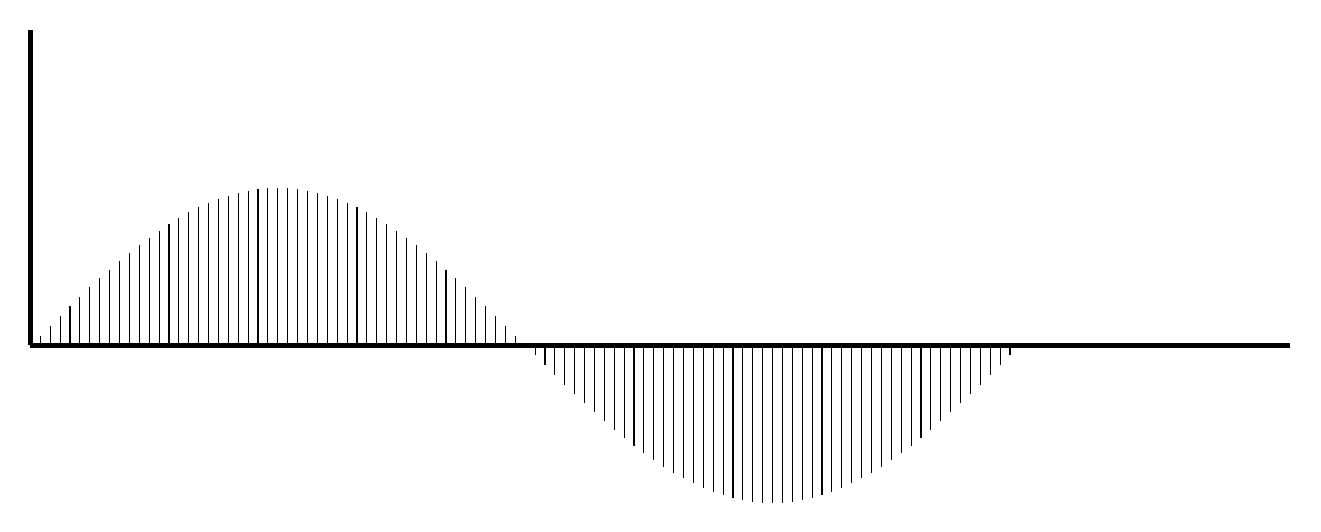
\begin{tikzpicture}[scale=2]

\draw[line width = 2] (0,0)--(8,0);
\draw[line width = 2] (0,0)--(0,2);

\draw (0.0,0)--(0.0,0.0);
\draw (0.0628318530718,0)--(0.0628318530718,0.0627905195293);
\draw (0.125663706144,0)--(0.125663706144,0.125333233564);
\draw (0.188495559215,0)--(0.188495559215,0.187381314586);
\draw (0.251327412287,0)--(0.251327412287,0.248689887165);
\draw (0.314159265359,0)--(0.314159265359,0.309016994375);
\draw (0.376991118431,0)--(0.376991118431,0.368124552685);
\draw (0.439822971503,0)--(0.439822971503,0.425779291565);
\draw (0.502654824574,0)--(0.502654824574,0.481753674102);
\draw (0.565486677646,0)--(0.565486677646,0.535826794979);
\draw (0.628318530718,0)--(0.628318530718,0.587785252292);
\draw (0.69115038379,0)--(0.69115038379,0.637423989749);
\draw (0.753982236862,0)--(0.753982236862,0.684547105929);
\draw (0.816814089933,0)--(0.816814089933,0.728968627421);
\draw (0.879645943005,0)--(0.879645943005,0.770513242776);
\draw (0.942477796077,0)--(0.942477796077,0.809016994375);
\draw (1.00530964915,0)--(1.00530964915,0.844327925502);
\draw (1.06814150222,0)--(1.06814150222,0.876306680044);
\draw (1.13097335529,0)--(1.13097335529,0.904827052466);
\draw (1.19380520836,0)--(1.19380520836,0.929776485888);
\draw (1.25663706144,0)--(1.25663706144,0.951056516295);
\draw (1.31946891451,0)--(1.31946891451,0.968583161129);
\draw (1.38230076758,0)--(1.38230076758,0.982287250729);
\draw (1.44513262065,0)--(1.44513262065,0.992114701314);
\draw (1.50796447372,0)--(1.50796447372,0.998026728428);
\draw (1.57079632679,0)--(1.57079632679,1.0);
\draw (1.63362817987,0)--(1.63362817987,0.998026728428);
\draw (1.69646003294,0)--(1.69646003294,0.992114701314);
\draw (1.75929188601,0)--(1.75929188601,0.982287250729);
\draw (1.82212373908,0)--(1.82212373908,0.968583161129);
\draw (1.88495559215,0)--(1.88495559215,0.951056516295);
\draw (1.94778744523,0)--(1.94778744523,0.929776485888);
\draw (2.0106192983,0)--(2.0106192983,0.904827052466);
\draw (2.07345115137,0)--(2.07345115137,0.876306680044);
\draw (2.13628300444,0)--(2.13628300444,0.844327925502);
\draw (2.19911485751,0)--(2.19911485751,0.809016994375);
\draw (2.26194671058,0)--(2.26194671058,0.770513242776);
\draw (2.32477856366,0)--(2.32477856366,0.728968627421);
\draw (2.38761041673,0)--(2.38761041673,0.684547105929);
\draw (2.4504422698,0)--(2.4504422698,0.637423989749);
\draw (2.51327412287,0)--(2.51327412287,0.587785252292);
\draw (2.57610597594,0)--(2.57610597594,0.535826794979);
\draw (2.63893782902,0)--(2.63893782902,0.481753674102);
\draw (2.70176968209,0)--(2.70176968209,0.425779291565);
\draw (2.76460153516,0)--(2.76460153516,0.368124552685);
\draw (2.82743338823,0)--(2.82743338823,0.309016994375);
\draw (2.8902652413,0)--(2.8902652413,0.248689887165);
\draw (2.95309709437,0)--(2.95309709437,0.187381314586);
\draw (3.01592894745,0)--(3.01592894745,0.125333233564);
\draw (3.07876080052,0)--(3.07876080052,0.0627905195293);
\draw (3.14159265359,0)--(3.14159265359,1.22464679915e-16);
\draw (3.20442450666,0)--(3.20442450666,-0.0627905195293);
\draw (3.26725635973,0)--(3.26725635973,-0.125333233564);
\draw (3.33008821281,0)--(3.33008821281,-0.187381314586);
\draw (3.39292006588,0)--(3.39292006588,-0.248689887165);
\draw (3.45575191895,0)--(3.45575191895,-0.309016994375);
\draw (3.51858377202,0)--(3.51858377202,-0.368124552685);
\draw (3.58141562509,0)--(3.58141562509,-0.425779291565);
\draw (3.64424747816,0)--(3.64424747816,-0.481753674102);
\draw (3.70707933124,0)--(3.70707933124,-0.535826794979);
\draw (3.76991118431,0)--(3.76991118431,-0.587785252292);
\draw (3.83274303738,0)--(3.83274303738,-0.637423989749);
\draw (3.89557489045,0)--(3.89557489045,-0.684547105929);
\draw (3.95840674352,0)--(3.95840674352,-0.728968627421);
\draw (4.02123859659,0)--(4.02123859659,-0.770513242776);
\draw (4.08407044967,0)--(4.08407044967,-0.809016994375);
\draw (4.14690230274,0)--(4.14690230274,-0.844327925502);
\draw (4.20973415581,0)--(4.20973415581,-0.876306680044);
\draw (4.27256600888,0)--(4.27256600888,-0.904827052466);
\draw (4.33539786195,0)--(4.33539786195,-0.929776485888);
\draw (4.39822971503,0)--(4.39822971503,-0.951056516295);
\draw (4.4610615681,0)--(4.4610615681,-0.968583161129);
\draw (4.52389342117,0)--(4.52389342117,-0.982287250729);
\draw (4.58672527424,0)--(4.58672527424,-0.992114701314);
\draw (4.64955712731,0)--(4.64955712731,-0.998026728428);
\draw (4.71238898038,0)--(4.71238898038,-1.0);
\draw (4.77522083346,0)--(4.77522083346,-0.998026728428);
\draw (4.83805268653,0)--(4.83805268653,-0.992114701314);
\draw (4.9008845396,0)--(4.9008845396,-0.982287250729);
\draw (4.96371639267,0)--(4.96371639267,-0.968583161129);
\draw (5.02654824574,0)--(5.02654824574,-0.951056516295);
\draw (5.08938009882,0)--(5.08938009882,-0.929776485888);
\draw (5.15221195189,0)--(5.15221195189,-0.904827052466);
\draw (5.21504380496,0)--(5.21504380496,-0.876306680044);
\draw (5.27787565803,0)--(5.27787565803,-0.844327925502);
\draw (5.3407075111,0)--(5.3407075111,-0.809016994375);
\draw (5.40353936417,0)--(5.40353936417,-0.770513242776);
\draw (5.46637121725,0)--(5.46637121725,-0.728968627421);
\draw (5.52920307032,0)--(5.52920307032,-0.684547105929);
\draw (5.59203492339,0)--(5.59203492339,-0.637423989749);
\draw (5.65486677646,0)--(5.65486677646,-0.587785252292);
\draw (5.71769862953,0)--(5.71769862953,-0.535826794979);
\draw (5.78053048261,0)--(5.78053048261,-0.481753674102);
\draw (5.84336233568,0)--(5.84336233568,-0.425779291565);
\draw (5.90619418875,0)--(5.90619418875,-0.368124552685);
\draw (5.96902604182,0)--(5.96902604182,-0.309016994375);
\draw (6.03185789489,0)--(6.03185789489,-0.248689887165);
\draw (6.09468974796,0)--(6.09468974796,-0.187381314586);
\draw (6.15752160104,0)--(6.15752160104,-0.125333233564);
\draw (6.22035345411,0)--(6.22035345411,-0.0627905195293);

\end{tikzpicture} \\ \\
\noindent This is the plot of a sine curve.  There's already an enormouse amount of content here.  If you don't like the Python programming language, feel free to use the language of your choice:

\begin{verbatim}
import numpy as np
x = 2*np.pi*np.arange(0,1,0.01)

for y in np.vstack((x, x,np.sin(x))).T:
	     print "\draw (%s,0)--(%s,%s);"%(y)

\end{verbatim}
The reason we want to engage in such plotting today, is to figure out what the book is talking about.  In the course of proving the Prime Number Theorem, three kernels are mentioned:
\begin{itemize}
\item $\displaystyle D_T(x) = \frac{\sin \pi T x}{\pi T x}$ Dirichlet Kernel
\item $\displaystyle \Delta_T(x) = T \left( \frac{\sin \pi T x}{\pi T x} \right)^2$ Fejer kernel
\item $\displaystyle J_T(x) = \frac{3T}{4} \left( \frac{\sin \pi T x}{\pi T x} \right)^4$ Jackson kernel
\end{itemize}
The questions we're asking are really basic.  What is a kernel?  What do they do in general?  How did they help us solve the Prime Number Theorem?  \\ \\
The first two theorems have to do with the pointwise convergence of Fourier series, and other things which we took for granted should be true 100\% of the time.  The last kernel has to do with the ``modulus of continuity" of the function.  \\ \\
All of these theorems require Lebesgue integration - and we know it doens't get any easier - so what are these functions $f(x)$ and subsets of $\mathbb{R}$ that are so complicated?  The function in question in PNT is:
$$ \frac{\zeta'(s)}{\zeta(s)}  - \frac{1}{1-s} = \sum \Lambda(n) \, n^{-s} - \frac{1}{1-s} \text{ with }\zeta(s) = \sum_{n =1}^\infty \frac{1}{n^s} 
\text{ and }\Lambda(n) = \left\{
\begin{array}{cc}
\log p & n = p^k \\
0 & \text{otherwise} \end{array} \right. $$
In order for us to be using Lebesgue measure, there must be subsets of $\mathbb{Z}$ that are pretty  hard to describe.

\begin{tikzpicture}[yscale=1]

\draw[line width = 1] (-5,0)--(5,0);
\draw[line width = 1] (0,-3)--(0,6);

\draw (-6.25176938064,0)--(-6.25176938064,-0.0250224305338);
\draw (-6.18893752757,0)--(-6.18893752757,-0.0733551595435);
\draw (-6.1261056745,0)--(-6.1261056745,-0.115425168738);
\draw (-6.06327382143,0)--(-6.06327382143,-0.146951391349);
\draw (-6.00044196836,0)--(-6.00044196836,-0.164602598576);
\draw (-5.93761011528,0)--(-5.93761011528,-0.166344425016);
\draw (-5.87477826221,0)--(-5.87477826221,-0.151666409253);
\draw (-5.81194640914,0)--(-5.81194640914,-0.121664367048);
\draw (-5.74911455607,0)--(-5.74911455607,-0.0789670296725);
\draw (-5.686282703,0)--(-5.686282703,-0.0275108490399);
\draw (-5.62345084993,0)--(-5.62345084993,0.027818232828);
\draw (-5.56061899685,0)--(-5.56061899685,0.0816438781359);
\draw (-5.49778714378,0)--(-5.49778714378,0.128616616594);
\draw (-5.43495529071,0)--(-5.43495529071,0.163939991505);
\draw (-5.37212343764,0)--(-5.37212343764,0.183854364491);
\draw (-5.30929158457,0)--(-5.30929158457,0.186030155787);
\draw (-5.24645973149,0)--(-5.24645973149,0.16983005108);
\draw (-5.18362787842,0)--(-5.18362787842,0.136411563054);
\draw (-5.12079602535,0)--(-5.12079602535,0.0886562357672);
\draw (-5.05796417228,0)--(-5.05796417228,0.030928345815);
\draw (-4.99513231921,0)--(-4.99513231921,-0.0313173816114);
\draw (-4.93230046614,0)--(-4.93230046614,-0.092044372166);
\draw (-4.86946861306,0)--(-4.86946861306,-0.145212309058);
\draw (-4.80663675999,0)--(-4.80663675999,-0.185370055754);
\draw (-4.74380490692,0)--(-4.74380490692,-0.208205935947);
\draw (-4.68097305385,0)--(-4.68097305385,-0.211000646497);
\draw (-4.61814120078,0)--(-4.61814120078,-0.192936180479);
\draw (-4.55530934771,0)--(-4.55530934771,-0.155226951062);
\draw (-4.49247749463,0)--(-4.49247749463,-0.101055709301);
\draw (-4.42964564156,0)--(-4.42964564156,-0.0353153452214);
\draw (-4.36681378849,0)--(-4.36681378849,0.035823479685);
\draw (-4.30398193542,0)--(-4.30398193542,0.105481506789);
\draw (-4.24115008235,0)--(-4.24115008235,0.166725243733);
\draw (-4.17831822927,0)--(-4.17831822927,0.213245252108);
\draw (-4.1154863762,0)--(-4.1154863762,0.23999310174);
\draw (-4.05265452313,0)--(-4.05265452313,0.243713925023);
\draw (-3.98982267006,0)--(-3.98982267006,0.223319830948);
\draw (-3.92699081699,0)--(-3.92699081699,0.180063263231);
\draw (-3.86415896392,0)--(-3.86415896392,0.117487531952);
\draw (-3.80132711084,0)--(-3.80132711084,0.0411525923654);
\draw (-3.73849525777,0)--(-3.73849525777,-0.0418442325733);
\draw (-3.6756634047,0)--(-3.6756634047,-0.12351253359);
\draw (-3.61283155163,0)--(-3.61283155163,-0.195720938295);
\draw (-3.54999969856,0)--(-3.54999969856,-0.250987774605);
\draw (-3.48716784548,0)--(-3.48716784548,-0.283235102054);
\draw (-3.42433599241,0)--(-3.42433599241,-0.288432076404);
\draw (-3.36150413934,0)--(-3.36150413934,-0.265061855424);
\draw (-3.29867228627,0)--(-3.29867228627,-0.214361027656);
\draw (-3.2358404332,0)--(-3.2358404332,-0.140300644952);
\draw (-3.17300858013,0)--(-3.17300858013,-0.0493016205566);
\draw (-3.11017672705,0)--(-3.11017672705,0.0502976128911);
\draw (-3.04734487398,0)--(-3.04734487398,0.148979035361);
\draw (-2.98451302091,0)--(-2.98451302091,0.236925346357);
\draw (-2.92168116784,0)--(-2.92168116784,0.304963640111);
\draw (-2.85884931477,0)--(-2.85884931477,0.345484575033);
\draw (-2.79601746169,0)--(-2.79601746169,0.353248273348);
\draw (-2.73318560862,0)--(-2.73318560862,0.325995615291);
\draw (-2.67035375555,0)--(-2.67035375555,0.264798916517);
\draw (-2.60752190248,0)--(-2.60752190248,0.174108029278);
\draw (-2.54469004941,0)--(-2.54469004941,0.0614748602002);
\draw (-2.48185819634,0)--(-2.48185819634,-0.0630311857749);
\draw (-2.41902634326,0)--(-2.41902634326,-0.187674888702);
\draw (-2.35619449019,0)--(-2.35619449019,-0.300105438719);
\draw (-2.29336263712,0)--(-2.29336263712,-0.388515322333);
\draw (-2.23053078405,0)--(-2.23053078405,-0.442804173634);
\draw (-2.16769893098,0)--(-2.16769893098,-0.455639077217);
\draw (-2.10486707791,0)--(-2.10486707791,-0.423307739259);
\draw (-2.04203522483,0)--(-2.04203522483,-0.346275506214);
\draw (-1.97920337176,0)--(-1.97920337176,-0.229380419525);
\draw (-1.91637151869,0)--(-1.91637151869,-0.0816305520691);
\draw (-1.85353966562,0)--(-1.85353966562,0.0843976894274);
\draw (-1.79070781255,0)--(-1.79070781255,0.253525726843);
\draw (-1.72787595947,0)--(-1.72787595947,0.409234689162);
\draw (-1.6650441064,0)--(-1.6650441064,0.535124877931);
\draw (-1.60221225333,0)--(-1.60221225333,0.616452869176);
\draw (-1.53938040026,0)--(-1.53938040026,0.641614210775);
\draw (-1.47654854719,0)--(-1.47654854719,0.603438692135);
\draw (-1.41371669412,0)--(-1.41371669412,0.500175731198);
\draw (-1.35088484104,0)--(-1.35088484104,0.336068986746);
\draw (-1.28805298797,0)--(-1.28805298797,0.121450333566);
\draw (-1.2252211349,0)--(-1.2252211349,-0.1276785558);
\draw (-1.16238928183,0)--(-1.16238928183,-0.390566660272);
\draw (-1.09955742876,0)--(-1.09955742876,-0.643083082969);
\draw (-1.03672557568,0)--(-1.03672557568,-0.859442985768);
\draw (-0.973893722613,0)--(-0.973893722613,-1.01416439768);
\draw (-0.911061869541,0)--(-0.911061869541,-1.08410676993);
\draw (-0.848230016469,0)--(-0.848230016469,-1.05043031594);
\draw (-0.785398163397,0)--(-0.785398163397,-0.900316316157);
\draw (-0.722566310326,0)--(-0.722566310326,-0.628302888264);
\draw (-0.659734457254,0)--(-0.659734457254,-0.237117317915);
\draw (-0.596902604182,0)--(-0.596902604182,0.26207703559);
\draw (-0.53407075111,0)--(-0.53407075111,0.850056848827);
\draw (-0.471238898038,0)--(-0.471238898038,1.5005271936);
\draw (-0.408407044967,0)--(-0.408407044967,2.18166296387);
\draw (-0.345575191895,0)--(-0.345575191895,2.85809966618);
\draw (-0.282743338823,0)--(-0.282743338823,3.49323292533);
\draw (-0.219911485751,0)--(-0.219911485751,4.05165979005);
\draw (-0.157079632679,0)--(-0.157079632679,4.50158158079);
\draw (-0.0942477796077,0)--(-0.0942477796077,4.81698881002);
\draw (-0.0314159265359,0)--(-0.0314159265359,4.97946367622);
\draw (0.0314159265359,0)--(0.0314159265359,4.97946367622);
\draw (0.0942477796077,0)--(0.0942477796077,4.81698881002);
\draw (0.157079632679,0)--(0.157079632679,4.50158158079);
\draw (0.219911485751,0)--(0.219911485751,4.05165979005);
\draw (0.282743338823,0)--(0.282743338823,3.49323292533);
\draw (0.345575191895,0)--(0.345575191895,2.85809966618);
\draw (0.408407044967,0)--(0.408407044967,2.18166296387);
\draw (0.471238898038,0)--(0.471238898038,1.5005271936);
\draw (0.53407075111,0)--(0.53407075111,0.850056848827);
\draw (0.596902604182,0)--(0.596902604182,0.26207703559);
\draw (0.659734457254,0)--(0.659734457254,-0.237117317915);
\draw (0.722566310326,0)--(0.722566310326,-0.628302888264);
\draw (0.785398163397,0)--(0.785398163397,-0.900316316157);
\draw (0.848230016469,0)--(0.848230016469,-1.05043031594);
\draw (0.911061869541,0)--(0.911061869541,-1.08410676993);
\draw (0.973893722613,0)--(0.973893722613,-1.01416439768);
\draw (1.03672557568,0)--(1.03672557568,-0.859442985768);
\draw (1.09955742876,0)--(1.09955742876,-0.643083082969);
\draw (1.16238928183,0)--(1.16238928183,-0.390566660272);
\draw (1.2252211349,0)--(1.2252211349,-0.1276785558);
\draw (1.28805298797,0)--(1.28805298797,0.121450333566);
\draw (1.35088484104,0)--(1.35088484104,0.336068986746);
\draw (1.41371669412,0)--(1.41371669412,0.500175731198);
\draw (1.47654854719,0)--(1.47654854719,0.603438692135);
\draw (1.53938040026,0)--(1.53938040026,0.641614210775);
\draw (1.60221225333,0)--(1.60221225333,0.616452869176);
\draw (1.6650441064,0)--(1.6650441064,0.535124877931);
\draw (1.72787595947,0)--(1.72787595947,0.409234689162);
\draw (1.79070781255,0)--(1.79070781255,0.253525726843);
\draw (1.85353966562,0)--(1.85353966562,0.0843976894274);
\draw (1.91637151869,0)--(1.91637151869,-0.0816305520692);
\draw (1.97920337176,0)--(1.97920337176,-0.229380419525);
\draw (2.04203522483,0)--(2.04203522483,-0.346275506214);
\draw (2.10486707791,0)--(2.10486707791,-0.423307739259);
\draw (2.16769893098,0)--(2.16769893098,-0.455639077217);
\draw (2.23053078405,0)--(2.23053078405,-0.442804173634);
\draw (2.29336263712,0)--(2.29336263712,-0.388515322333);
\draw (2.35619449019,0)--(2.35619449019,-0.300105438719);
\draw (2.41902634326,0)--(2.41902634326,-0.187674888702);
\draw (2.48185819634,0)--(2.48185819634,-0.0630311857749);
\draw (2.54469004941,0)--(2.54469004941,0.0614748602002);
\draw (2.60752190248,0)--(2.60752190248,0.174108029278);
\draw (2.67035375555,0)--(2.67035375555,0.264798916517);
\draw (2.73318560862,0)--(2.73318560862,0.325995615291);
\draw (2.79601746169,0)--(2.79601746169,0.353248273348);
\draw (2.85884931477,0)--(2.85884931477,0.345484575033);
\draw (2.92168116784,0)--(2.92168116784,0.304963640111);
\draw (2.98451302091,0)--(2.98451302091,0.236925346357);
\draw (3.04734487398,0)--(3.04734487398,0.148979035361);
\draw (3.11017672705,0)--(3.11017672705,0.0502976128911);
\draw (3.17300858013,0)--(3.17300858013,-0.0493016205566);
\draw (3.2358404332,0)--(3.2358404332,-0.140300644952);
\draw (3.29867228627,0)--(3.29867228627,-0.214361027656);
\draw (3.36150413934,0)--(3.36150413934,-0.265061855424);
\draw (3.42433599241,0)--(3.42433599241,-0.288432076404);
\draw (3.48716784548,0)--(3.48716784548,-0.283235102054);
\draw (3.54999969856,0)--(3.54999969856,-0.250987774605);
\draw (3.61283155163,0)--(3.61283155163,-0.195720938295);
\draw (3.6756634047,0)--(3.6756634047,-0.12351253359);
\draw (3.73849525777,0)--(3.73849525777,-0.0418442325732);
\draw (3.80132711084,0)--(3.80132711084,0.0411525923654);
\draw (3.86415896392,0)--(3.86415896392,0.117487531952);
\draw (3.92699081699,0)--(3.92699081699,0.180063263231);
\draw (3.98982267006,0)--(3.98982267006,0.223319830948);
\draw (4.05265452313,0)--(4.05265452313,0.243713925023);
\draw (4.1154863762,0)--(4.1154863762,0.23999310174);
\draw (4.17831822927,0)--(4.17831822927,0.213245252108);
\draw (4.24115008235,0)--(4.24115008235,0.166725243733);
\draw (4.30398193542,0)--(4.30398193542,0.105481506789);
\draw (4.36681378849,0)--(4.36681378849,0.035823479685);
\draw (4.42964564156,0)--(4.42964564156,-0.0353153452214);
\draw (4.49247749463,0)--(4.49247749463,-0.101055709301);
\draw (4.55530934771,0)--(4.55530934771,-0.155226951062);
\draw (4.61814120078,0)--(4.61814120078,-0.192936180479);
\draw (4.68097305385,0)--(4.68097305385,-0.211000646497);
\draw (4.74380490692,0)--(4.74380490692,-0.208205935947);
\draw (4.80663675999,0)--(4.80663675999,-0.185370055754);
\draw (4.86946861306,0)--(4.86946861306,-0.145212309058);
\draw (4.93230046614,0)--(4.93230046614,-0.092044372166);
\draw (4.99513231921,0)--(4.99513231921,-0.0313173816114);
\draw (5.05796417228,0)--(5.05796417228,0.030928345815);
\draw (5.12079602535,0)--(5.12079602535,0.0886562357673);
\draw (5.18362787842,0)--(5.18362787842,0.136411563054);
\draw (5.24645973149,0)--(5.24645973149,0.16983005108);
\draw (5.30929158457,0)--(5.30929158457,0.186030155787);
\draw (5.37212343764,0)--(5.37212343764,0.183854364491);
\draw (5.43495529071,0)--(5.43495529071,0.163939991505);
\draw (5.49778714378,0)--(5.49778714378,0.128616616594);
\draw (5.56061899685,0)--(5.56061899685,0.0816438781359);
\draw (5.62345084993,0)--(5.62345084993,0.027818232828);
\draw (5.686282703,0)--(5.686282703,-0.0275108490399);
\draw (5.74911455607,0)--(5.74911455607,-0.0789670296725);
\draw (5.81194640914,0)--(5.81194640914,-0.121664367048);
\draw (5.87477826221,0)--(5.87477826221,-0.151666409253);
\draw (5.93761011528,0)--(5.93761011528,-0.166344425016);
\draw (6.00044196836,0)--(6.00044196836,-0.164602598576);
\draw (6.06327382143,0)--(6.06327382143,-0.146951391349);
\draw (6.1261056745,0)--(6.1261056745,-0.115425168738);
\draw (6.18893752757,0)--(6.18893752757,-0.0733551595435);
\draw (6.25176938064,0)--(6.25176938064,-0.0250224305337);



\end{tikzpicture} \\ \\
Arithmetically, what is the Dirichlet kernel doing?  Why does it not prove the Prime Number Theorem as readily as we'd like to. \\ \\
Dirichlet, Fejer, Jackson kernels are all called \textbf{Approximations to the Identity}, what is to say $D_T \asymp 1$, and yet $D_T \ast f$ is compactly supported.  Truth be told, they all look kind of the same to me.\\ \\
This seems like an awful amount of work, and I don't get an explanation of any of the parts in the middle, so I guess I'll do it myself. \\ \\
\textbf{Thm} (Stein) A family of Kernels $K_n(x)$ is called a ``good kernel" if 
\begin{itemize}
\item $\displaystyle \int_{-\pi}^\pi K_n(x) \, dx = 2\pi$ for all $n \geq 1$
\item $\displaystyle \int_{-\pi}^\pi |K_n(x) | \, dx \leq M$ for all $n \geq 1$ 
\item $\displaystyle \int_{\delta\leq |x|\leq \pi} |K_n(x)| \, dx \to 0$ as $n \to \infty$
\end{itemize}
\textbf{Thm} (Stein) Let $\{ K_n\}_{n=1}^\infty$ be a family of good kernels and $f$ be an Riemann integrable function on the circle then 
$$ \lim_{n \to \infty} (f*K_n)(x) = f(x) $$
whenever $f$ is continuous at $x$.  If $f$ is continuous everywhere, then the above limit is uniform. \\ \\
We need even more statements of these convergence theorems because our function is not continuous.  It'd be good to ask what goes wrong at all these discontinuities.  Fejer's theorem works when you have one or two\dots Our zeta function example, has countably many of discontinuities. \\ \\
\textbf{Dirichlet Kernel} Over $\mathbb{Z}$ we can write the partial sums of the Fourier series (as if it were always true)
$$ f(x) = \lim_{N \to \infty} \sum_{n=-N}^n \hat{f}(n)e^{2\pi i \, nx} = \sum_{n \in \mathbb{Z}} \langle f | n \rangle \langle n | x \rangle  = \langle f | x \rangle $$
So\dots we can make this statement look really really reasonable.  Too bad it's false.  The exceptions to this equation are fascinating things and that's why we have Lebesgue measure.   \\ \\
Here is the formula for the Dirichlet Kernel and we use the geometric serires formula:
$$ D_N(x) = \sum_{n = -N}^N e^{i n x} = \frac{\sin (N + \frac{1}{2})x}{\sin x/2} \text{ so that } (D_N * f)(x) = \sum_{n = - N}^N \hat{f}(n) \, e^{inx}$$
This represents the most common-sense way of adding a series of numbers that is infinite over both directions. \\ \\
What's good about ?  What's bad about it?
\vfill
\begin{thebibliography}{} 

\item Henri Cohen \textbf{Computational Number Theory in Relation with L-Functions} \texttt{arXiv:1809.10904}

\item Hugh Montgomery, Robert Vaughan \textbf{Multiplicative Number Theory I: Classical Theory} \\ (Cambridge Studies in Advanced Mathematics, \#97) Cambridge University Press, 2010.

\item Yitzhak Katznelson \textbf{An Introduction to Harmonic Analysis} (Cambridge Mathematical Library) \\ Cambridge University Press, 2004.

\end{thebibliography}

\end{document}